\newpage

\section{Figures}

\listoffigures

\begin{figure}[h]
  \centering
  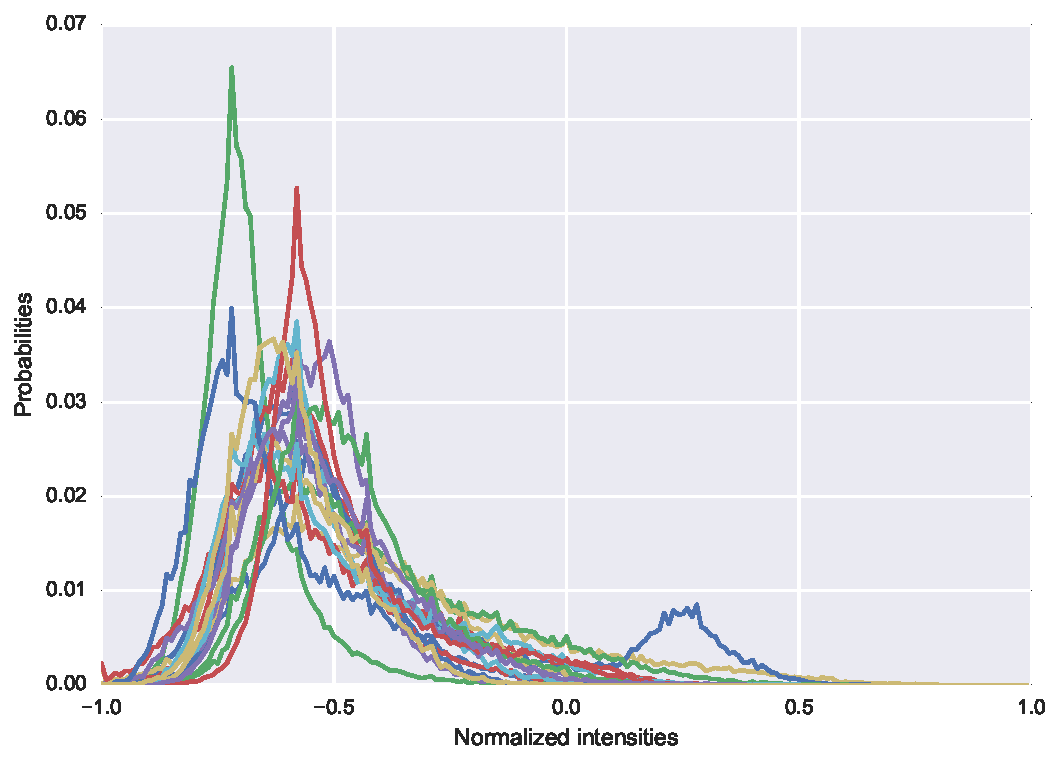
\includegraphics[width=0.7\linewidth]{02_methods/figures/t2w.pdf}
  \caption{Illustration of the inter-patient variations in 17 different patients, using the \acs*{pdf} representation.}
  \label{fig:t2w}
\end{figure}

\begin{figure*}
  \centering
  \hspace*{\fill}
  \subfigure[]{\label{subfig:pathhist}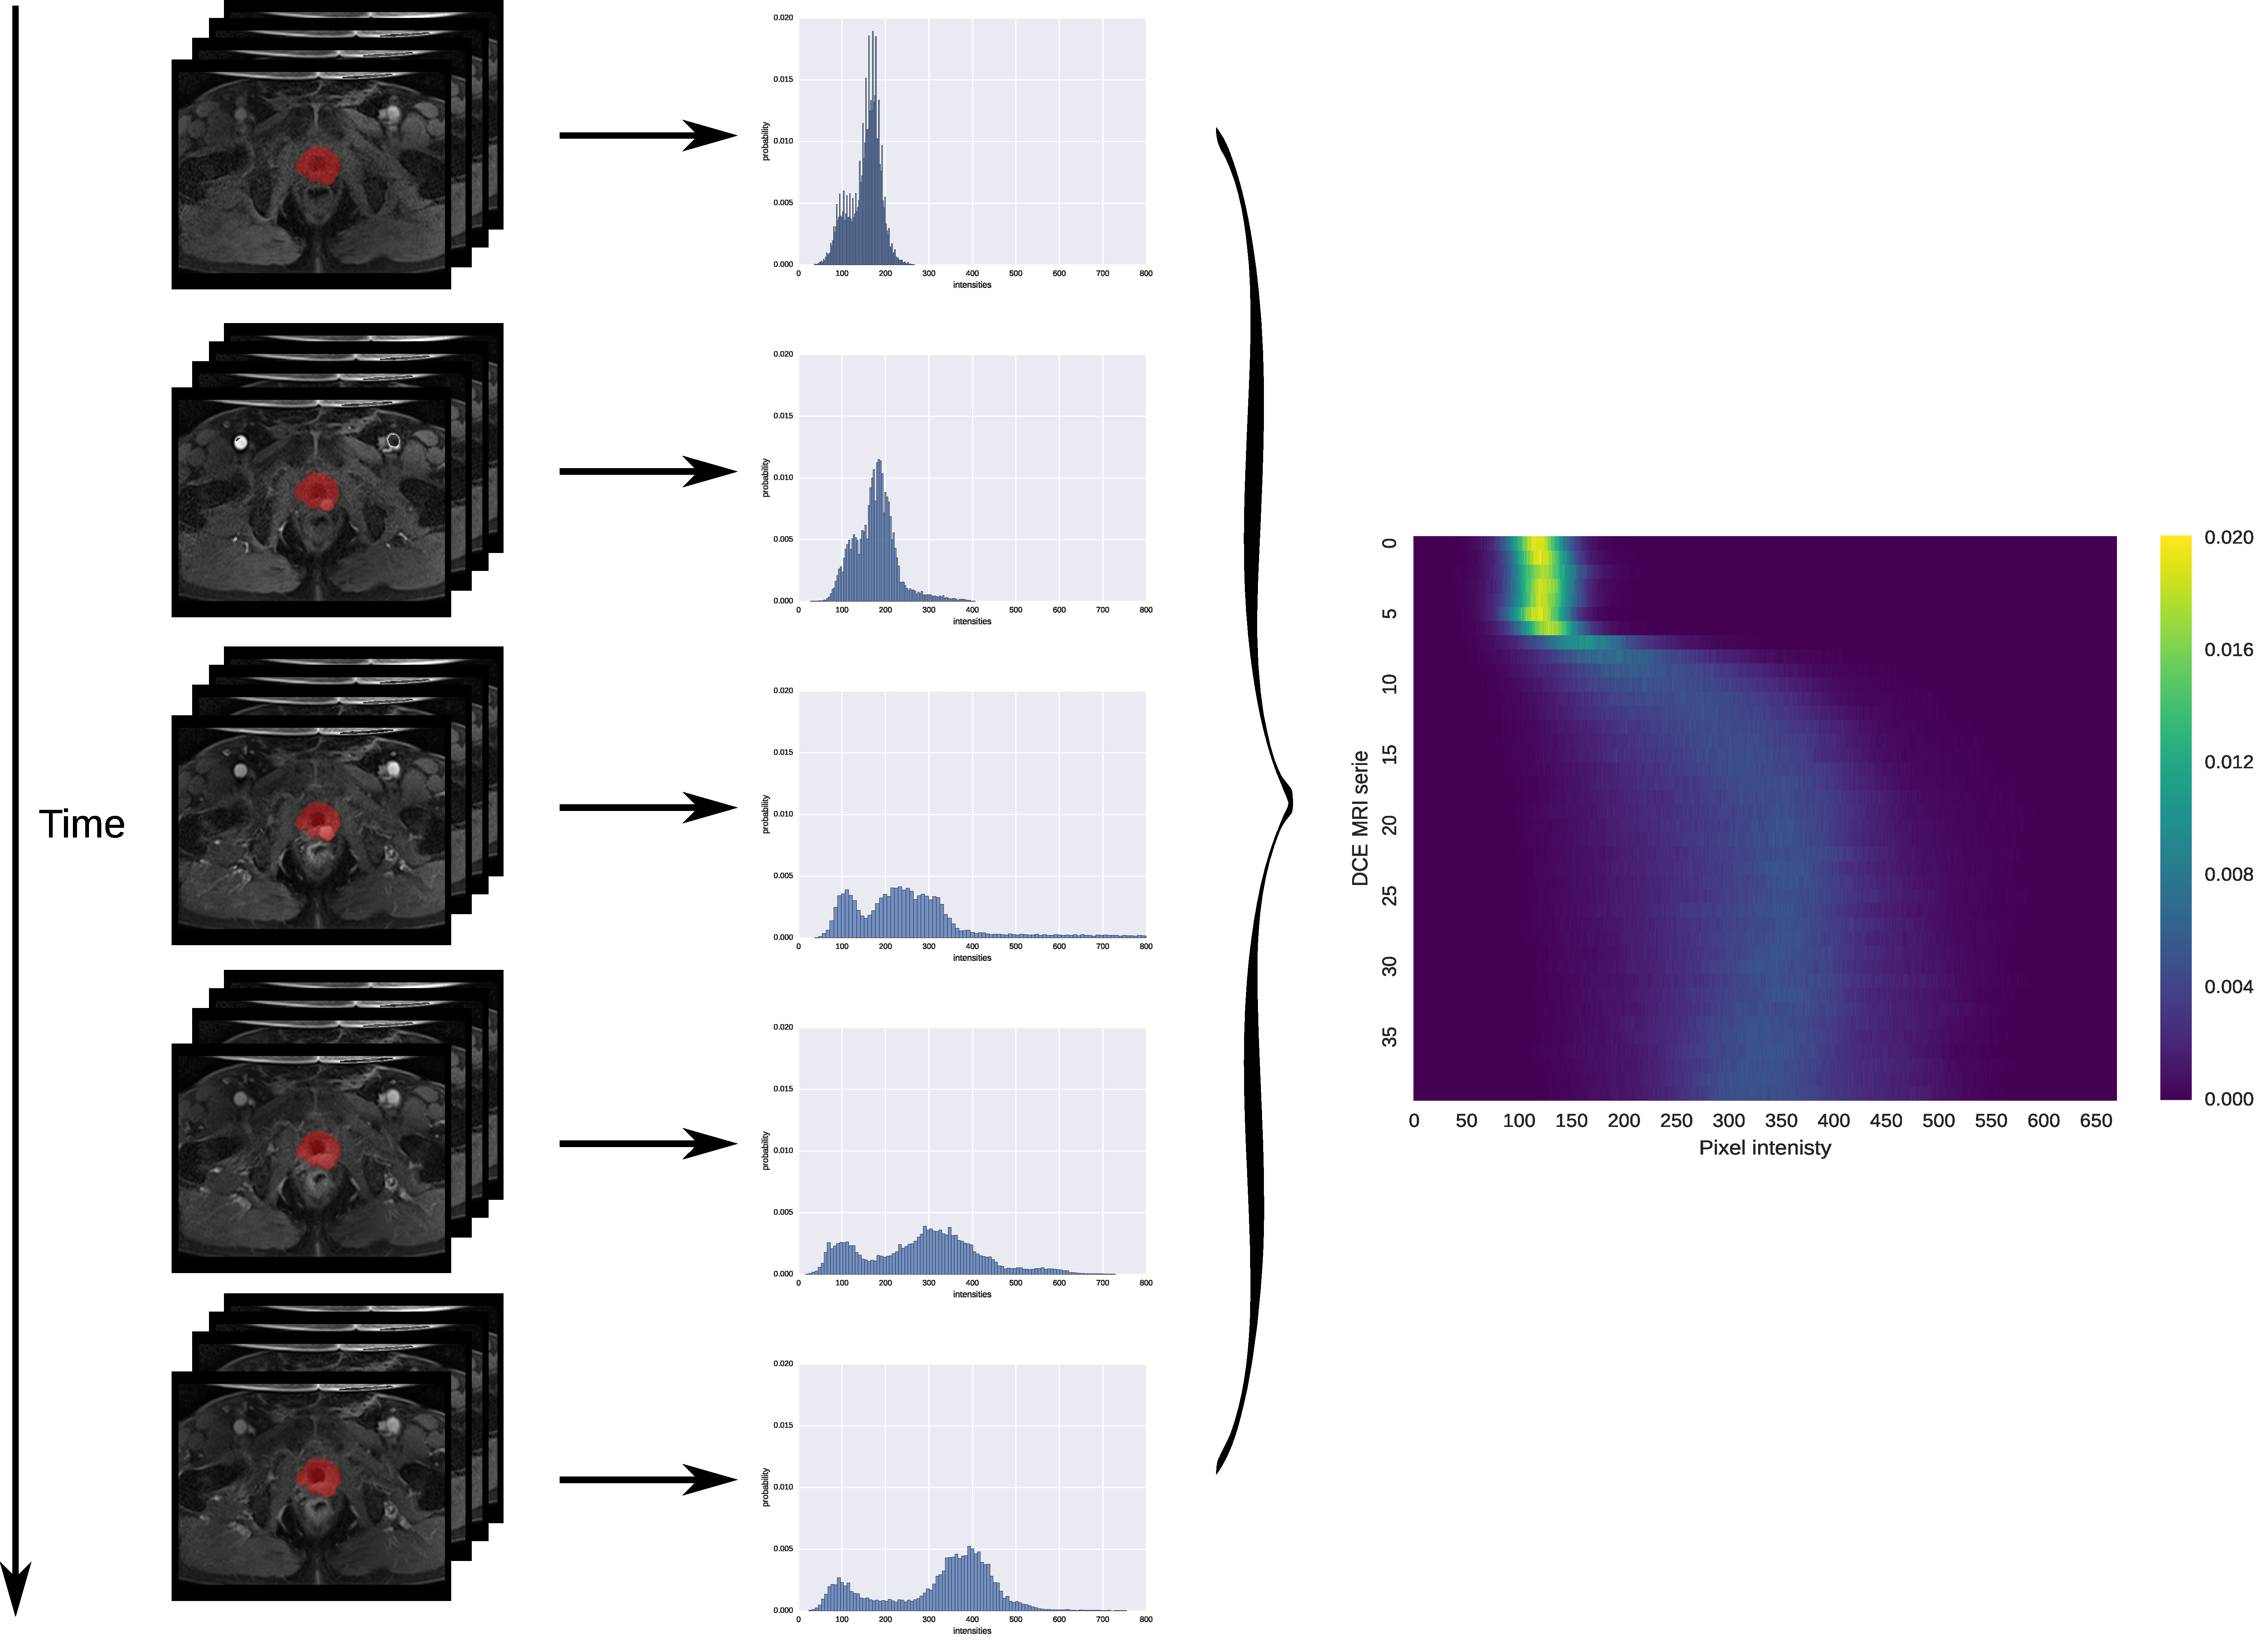
\includegraphics[width=1\textwidth]{02_methods/figures/heatmaprep.pdf}} \hfill
  \hspace*{\fill}
  \\
  \hspace*{\fill}
  \subfigure[]{\label{subfig:pat1}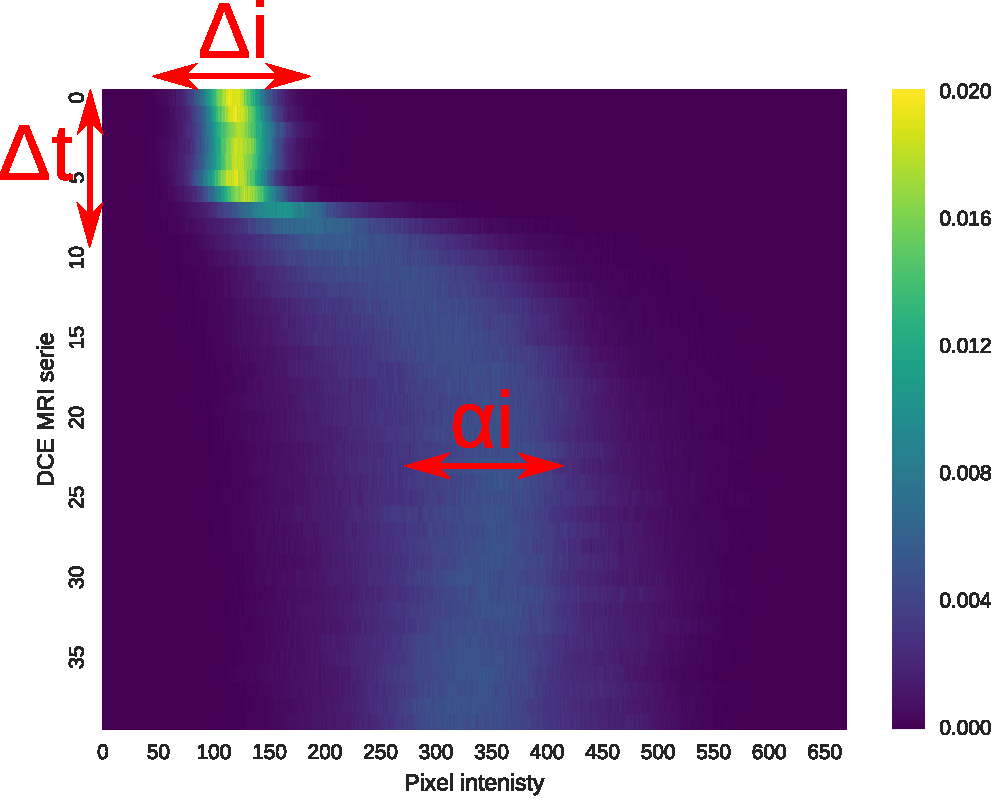
\includegraphics[width=.49\textwidth]{02_methods/figures/pat1_annotated.pdf}} \hfill
  \subfigure[]{\label{subfig:pat2}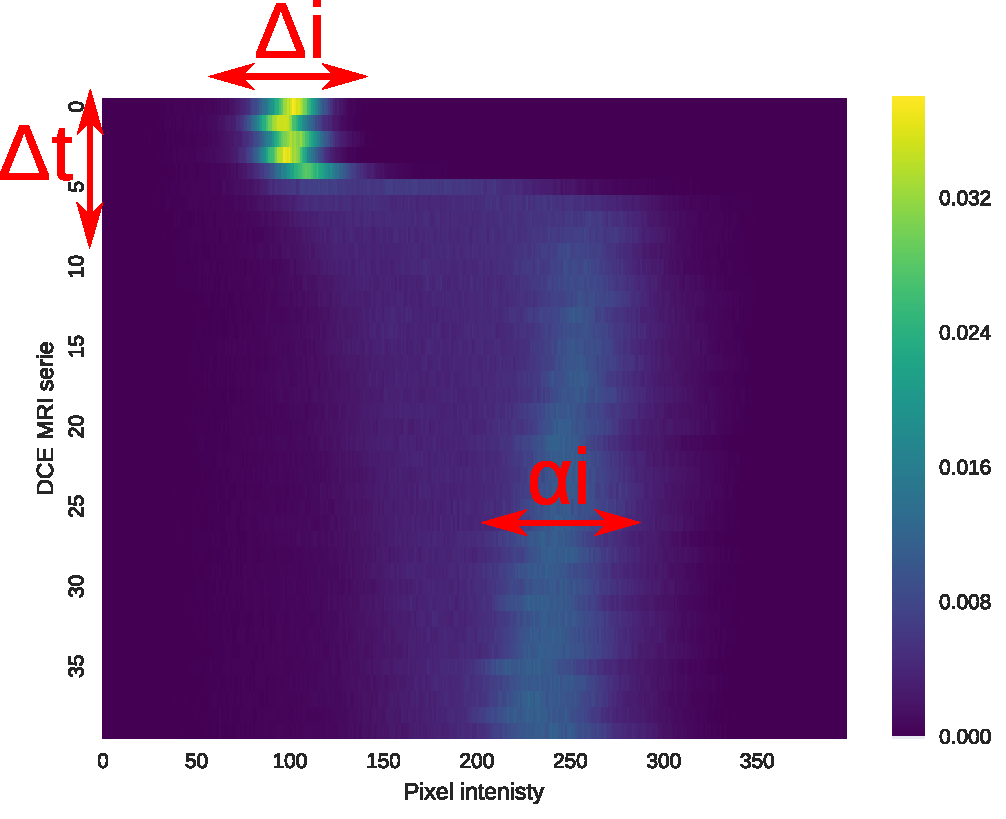
\includegraphics[width=.49\textwidth]{02_methods/figures/pat2_annotated.pdf}} \hfill
  \hspace*{\fill}
  \caption{\subref{subfig:pathhist} Illustration of the heatmap representation: all \ac*{pdf}s of the prostate gland are concatenated together to build an heatmap; \subref{subfig:pat1}-\subref{subfig:pat2} Illustration of inter-patient variations (i.e., $\Delta_i$, $\Delta_t$, and $\alpha_i$) \acs*{pdf} over time of two patients in a \ac{dce}-\ac{mri}.}
  \label{fig:heatmap}
\end{figure*}

\begin{figure}[h]
  \centering
  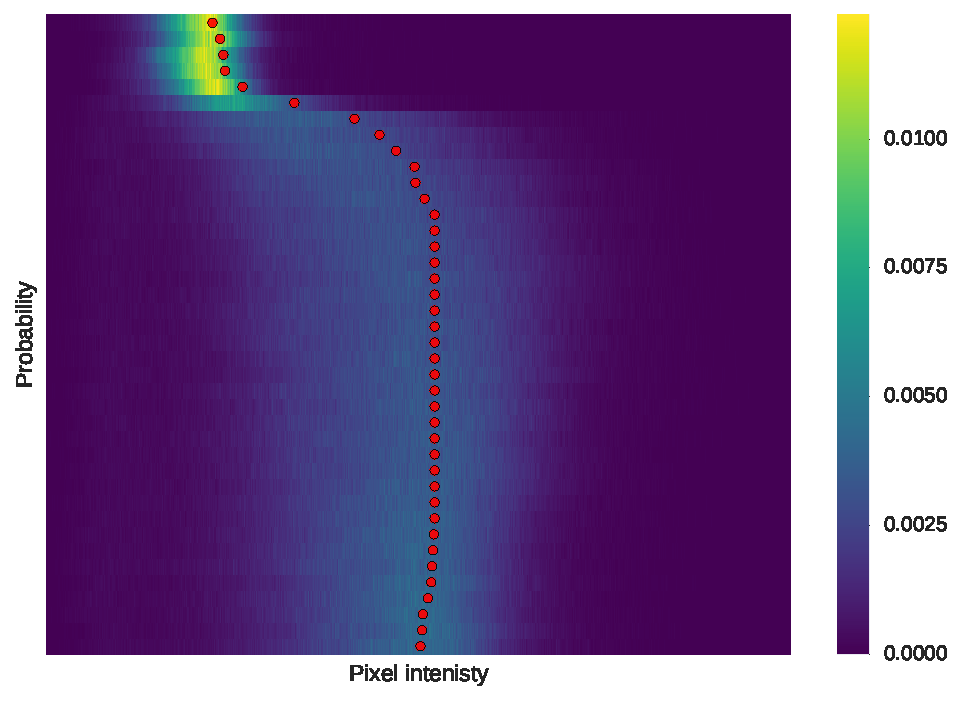
\includegraphics[width=0.7\linewidth]{02_methods/figures/estimator.pdf}
  \caption{Illustration of the estimator found using the shortest-path through the graph.}
  \label{fig:estimator}
\end{figure}

\begin{figure*}[h]
  \centering
  \hspace*{\fill}
  \subfigure[\acs*{rmse} computed for each patient of our dataset.]{\label{fig:rmse}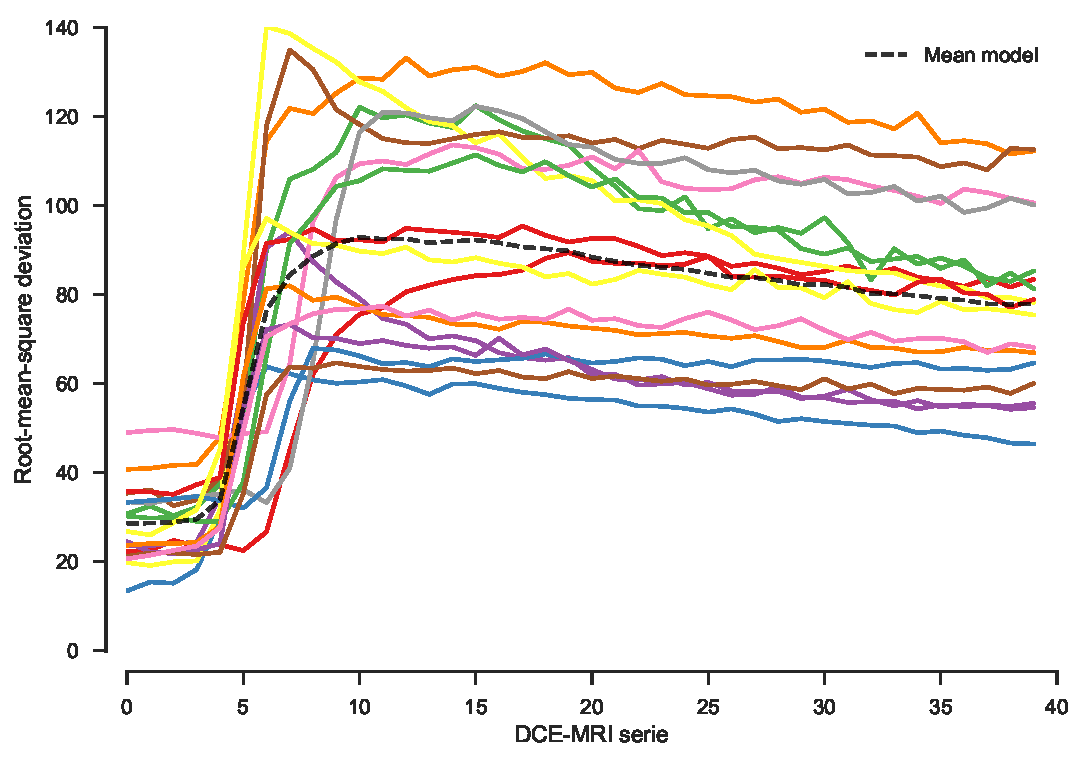
\includegraphics[width=.49\textwidth]{02_methods/figures/rmse.pdf}} \hfill
  \subfigure[\acs*{rmse} after alignment using the curve parametric model.]{\label{fig:rmseal}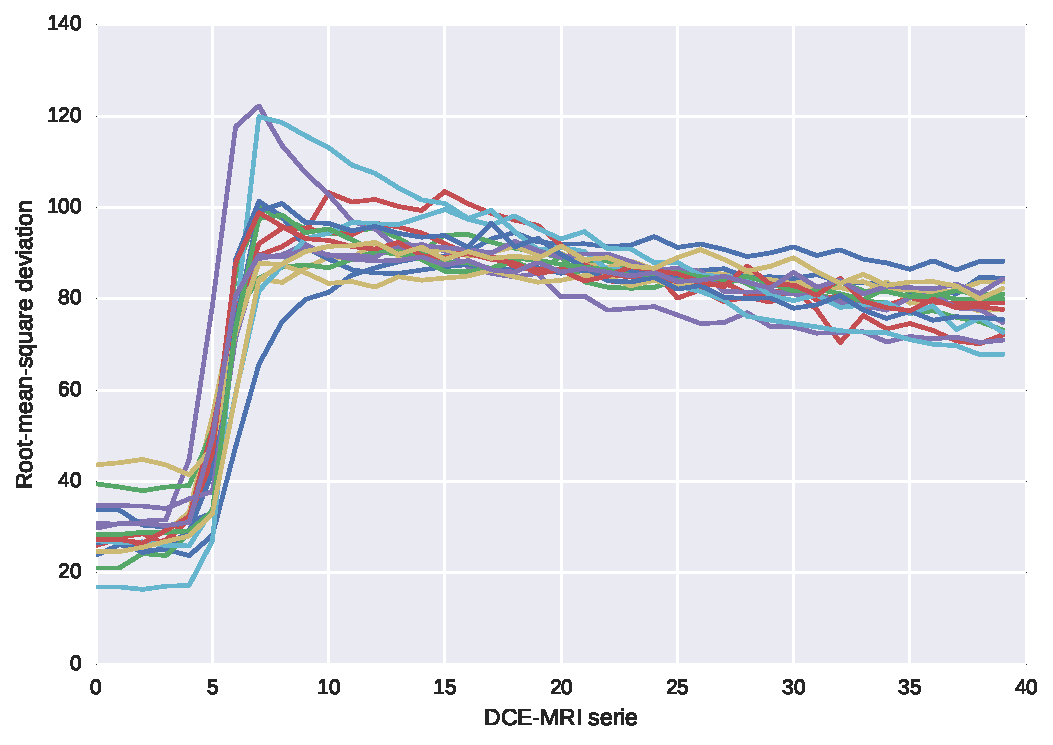
\includegraphics[width=.49\textwidth]{02_methods/figures/rmse_aligned.pdf}}
  \hspace*{\fill}
  \caption{Illustration of the correction of the time offset and the data dispersion.}
  \label{fig:curveal}
\end{figure*}

\begin{figure*}[h]
  \centering
  \hspace*{\fill}
  \subfigure[Original image.]{\label{fig:org}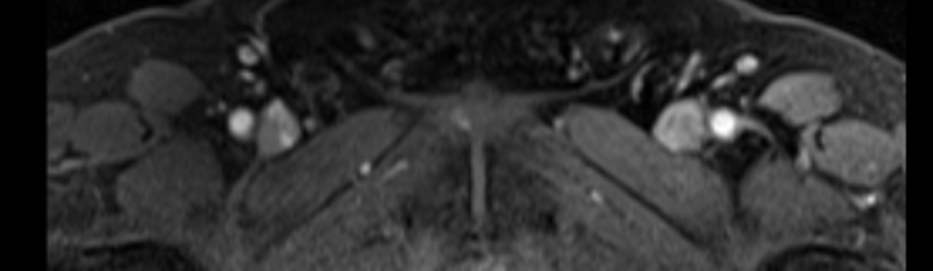
\includegraphics[width=.3\textwidth]{02_methods/figures/original.pdf}} \hfill
  \subfigure[Candidates region after clustering.]{\label{fig:cand}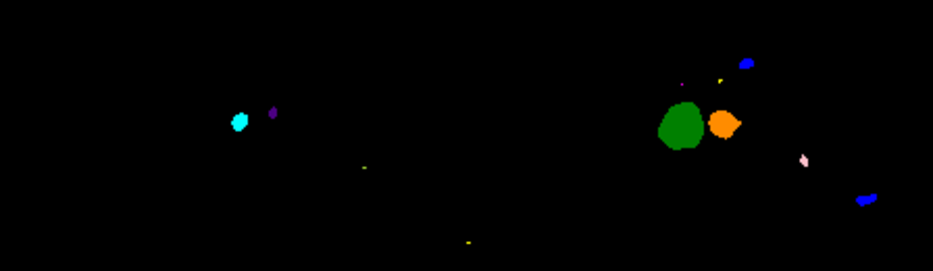
\includegraphics[width=.3\textwidth]{02_methods/figures/candidate.pdf}} \hfill
  \subfigure[Regions selected after applying the different criteria.]{\label{fig:final}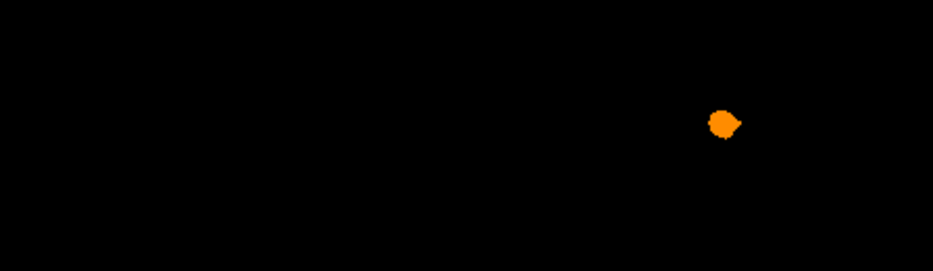
\includegraphics[width=.3\textwidth]{02_methods/figures/aif.pdf}}
  \hspace*{\fill}
  \caption{Illustration of the segmentation of the area used to determine the \acs*{aif}.}
  \label{fig:aif}
\end{figure*}

\begin{figure*}[h]
  \centering
  \hspace*{\fill}
  \subfigure[Without normalization.]{\label{fig:rfpharmaunorm}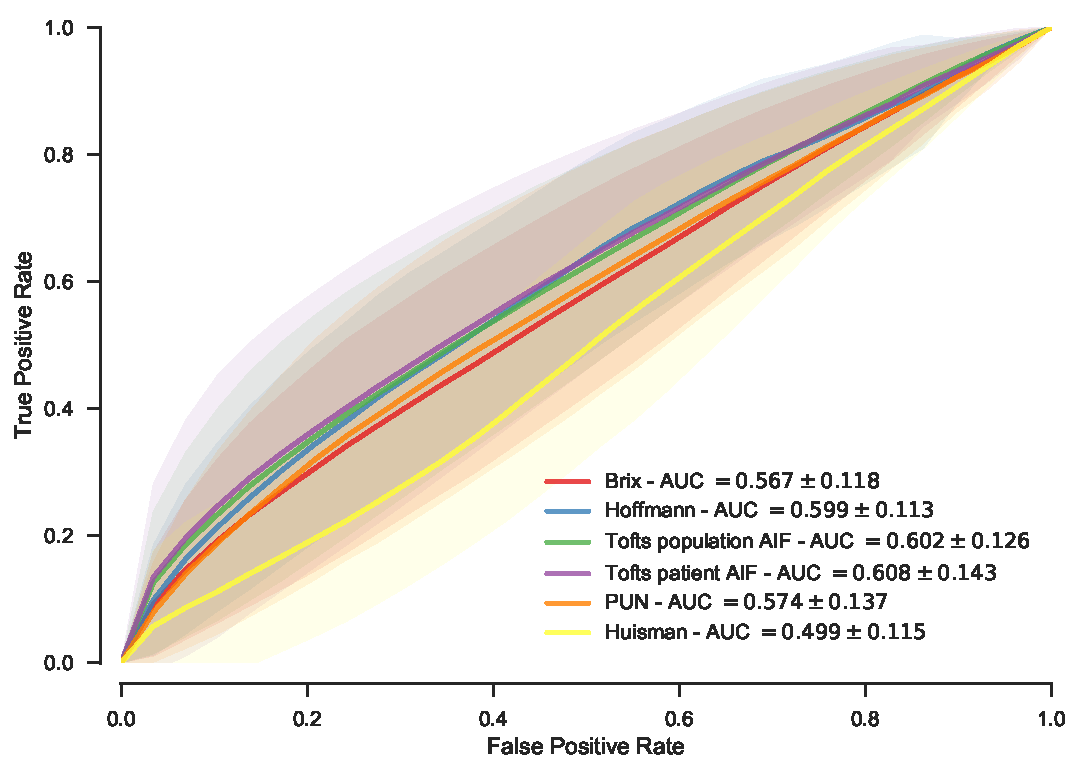
\includegraphics[width=.49\textwidth]{03_experiments/figures/unormalized/unormalized_methods_0.pdf}} \hfill
  \subfigure[With normalization.]{\label{fig:rfpharmanorm}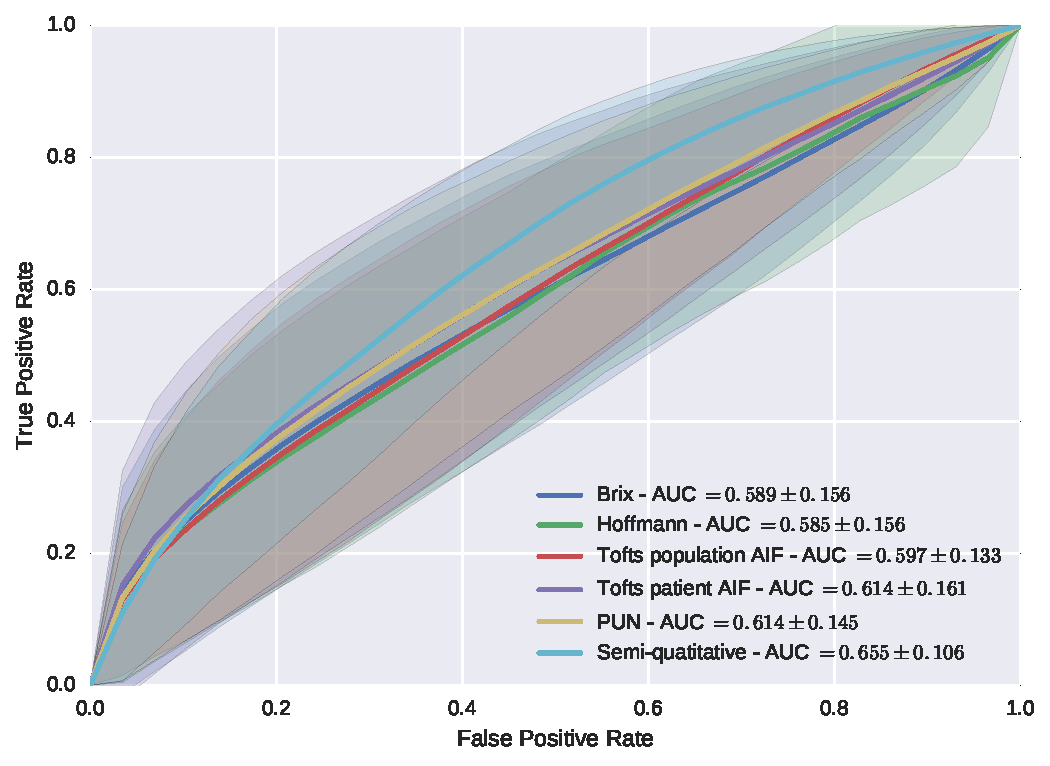
\includegraphics[width=.49\textwidth]{03_experiments/figures/normalized/normalized_methods_0.pdf}}
  \hspace*{\fill}
  \caption{\acs*{roc} analysis using a \acs*{rf} classifier with and without normalization \ac{dce}-\ac{mri} data for different pharmacokinetic models.}
  \label{fig:normpharmarf}
\end{figure*}

\begin{figure}[h]
  \centering
  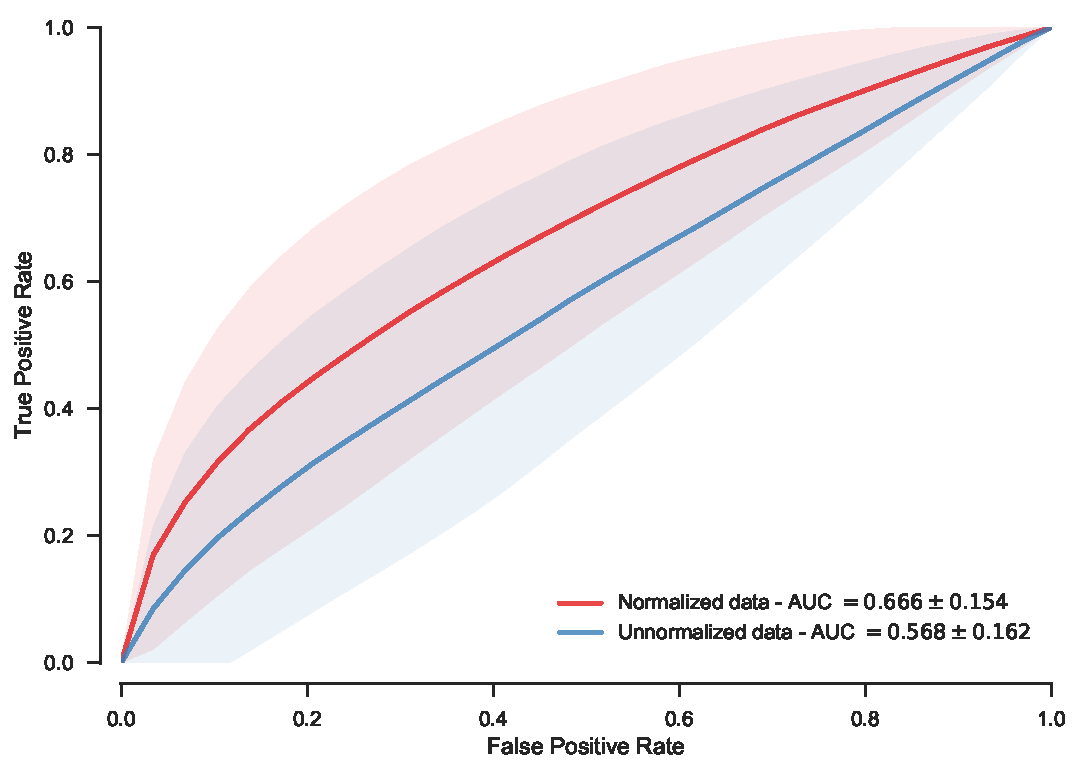
\includegraphics[width=0.7\linewidth]{03_experiments/figures/full_signal_0.pdf}
  \caption{\acs*{roc} analysis using the entire \ac{dce}-\ac{mri} signal with and without normalization in conjunction with a \acs*{rf} classifier.}
  \label{fig:rfnormdcesignal}
\end{figure}

%%% Local Variables: 
%%% mode: latex
%%% TeX-master: "../main"
%%% End: 
